\chapter{Gradient Based Optimization}
L'ottimizzazione è il processo di minimizzare o massimizzare una funzione $f(x)$ alterando il valore di $x$.
La funzione che vogliamo ottimizzare si chiama funzione obiettivo. La soluzione ottima viene denotata $x^*=\text{arg opt }f(x)$, $opt = \{min, max\} $.

Possiamo trovare i punti di massimo e minimo analiticamente ponendo il gradiente della funzione pari a zero $\nabla_x f(x^*) = 0$.

Nel caso di modelli lineari possiamo usare l'ottimizzazione convessa, mentre per quelli non lineari è necessario
usare una procedura iterativa di ottimizzazione numerica che trovano solo una approssimazione.

\section{Gradient Descent}
Il gradient descent (discesa del gradiente) è un algoritmo di ottimizzazione iterativo per trovare il minimo di una funzione differenziabile $f(x)$.

Ad ogni iterazione ci si muove da un punto iniziale $x_i$ nella direzione opposta a quella di massima crescita della funzione, ovvero $-\nabla_x f(x_i)$.
%
\begin{align*}
  x_{i+1} = x_i - \eta \nabla_x f(x_i)
\end{align*}
Il parametro $\eta$ controlla l'intensità dello spostamento (Figura \ref{fig:learning-rate}). Per valori molto piccoli la convergenza sarà lenta, mentre per valori troppo grandi si rischia di arrivare
in un ottimo locale sub ottimale.

L'algoritmo si ferma in base a un criterio specificato ad esempio quando lo spostamento diventa molto piccolo o dopo un numero predefinito di iterazioni.
\begin{figure}
  \centering
  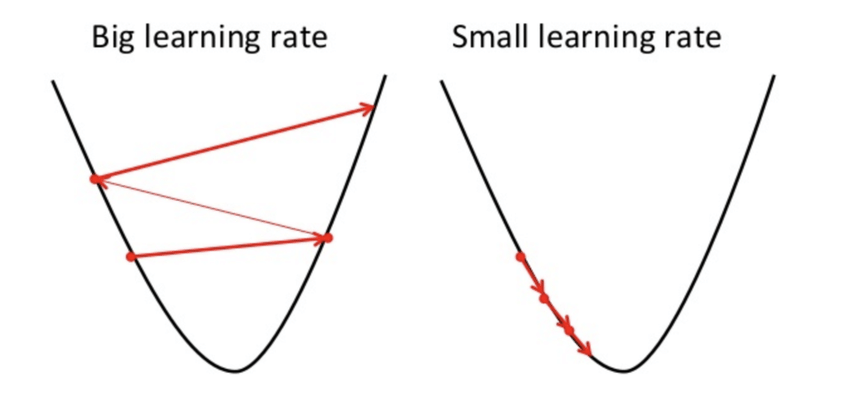
\includegraphics[width=0.8\linewidth]{images/learning-rate.png}
  \caption{Comportamento del gradient descent con valori alti e bassi di $\eta$ \cite{img:learning-rate}.}
  \label{fig:learning-rate}
\end{figure}

\section{Training as Optimization}
L'obiettivo di un algoritmo di training è quello di ritornare una funzione $f(x)$ che mappa con una certa accuratezza gli input $x$
alle etichette corrispondenti $y$.

Per valutare l'accuratezza della funzione $f(x)$ introduciamo il concetto di loss function.

La funzione di loss $L(y, \hat{y})$ assegna uno score numerico (scalare) all'output predetto $\hat{y}$ dato il valore di verità atteso $y$.

I parametri della funzione $f(x; \theta)$ sono scelti in modo da minimizzare la loss $L$ sugli esempi di training.

Dato un training set etichettato $(x_{1:n}, y_{1:n})$, una funzione di loss $L$ e una funzione parametrica $f(x; \theta)$, denotiamo la \textbf{cost function} come segue:
\begin{align*}
  J(\theta) = \frac{1}{n} \sum_{i=1}^n L(x_i, y_i; \theta)
\end{align*}

L'obiettivo dell'algoritmo di training è quindi impostare i parametri $\theta$ in modo che il valore di $J(\theta)$ sia minimizzato.
\begin{align*}
  \hat{\theta} = \underset{\theta}{\mathrm{argmin}}{J(\theta)}
\end{align*}

\newpage

\section{Stochastic, Batch, Mini-Batch}
La cost function viene spesso decomposta come somma delle loss calcolate sui singoli esempi.
\begin{align*}
  J(\theta) = \mathbb{E}_{x,y\sim\hat{p}_{data}} L(x, y; \theta) = \frac{1}{n} \sum_{i=1}^n L(x_i, y_i; \theta)
\end{align*}
%
Il gradiente della loss $J(\theta)$ può essere calcolato come media dei gradienti delle singole loss.
\begin{align*}
  \nabla_\theta J(\theta) = \frac{1}{n} \sum_{i=1}^n \nabla_\theta L(x_i, y_i; \theta)
\end{align*}
%
Tuttavia calcolare il gradiente per ogni esempio può essere costoso per $n$ grandi, in quanto il costo è lineare nel numero di esempi.

Possiamo quindi usare un insieme di $m$ esempi $B = \{x^1, x^2, ..., X^m\}$ che viene detto \textbf{minibatch}.
\begin{align*}
  g = \frac{1}{m} \sum_{i=1}^m \nabla_\theta L(x_i, y_i; \theta)
\end{align*}

Gli algoritmi di gradient descent prendono un nome diverso in base a quanti esempi vengono utilizzati per calcolare il gradiente della funzione di costo (Figura \ref{fig:gradient-descent}).

\begin{figure}[h]
  \centering
  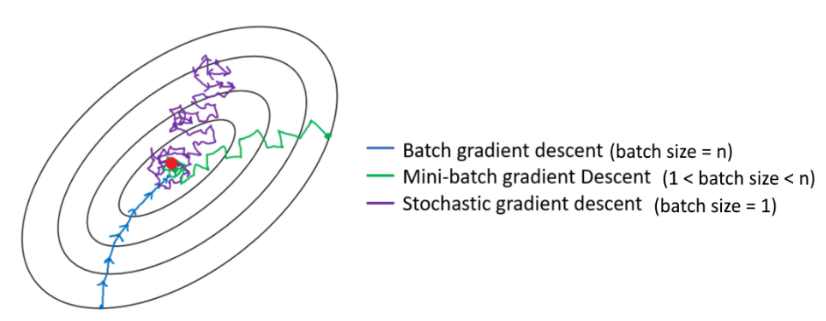
\includegraphics[width=0.9\linewidth]{images/gradient-descent.png}
  \caption{Rappresentazione del gradient descent con diverse batch size \cite{img:gradient-descent}.}
  \label{fig:gradient-descent}
\end{figure}

Con un numero di batch grande si ottiene una stima migliore, mentre con batch piccole una convergenza veloce.
Solitamente le dimensioni scelte per la minibatch sono potenze di 2 (8, 16, 32, 64, ...) per sfruttare il calcolo parallelo su GPU.

Il numero di aggiornamenti per arrivare alla convergenza aumenta con in numero di esempi.
L'aggiornamento del modello non dipende dal numero di esempi.

\section{Empirical Risk}

\section{Ill Conditioning}

\section{Local Minima}

\section{Altri Algoritmi}
